\documentclass[14pt]{extreport}
\usepackage{gost}

\begin{document}

\pagestyle{empty}
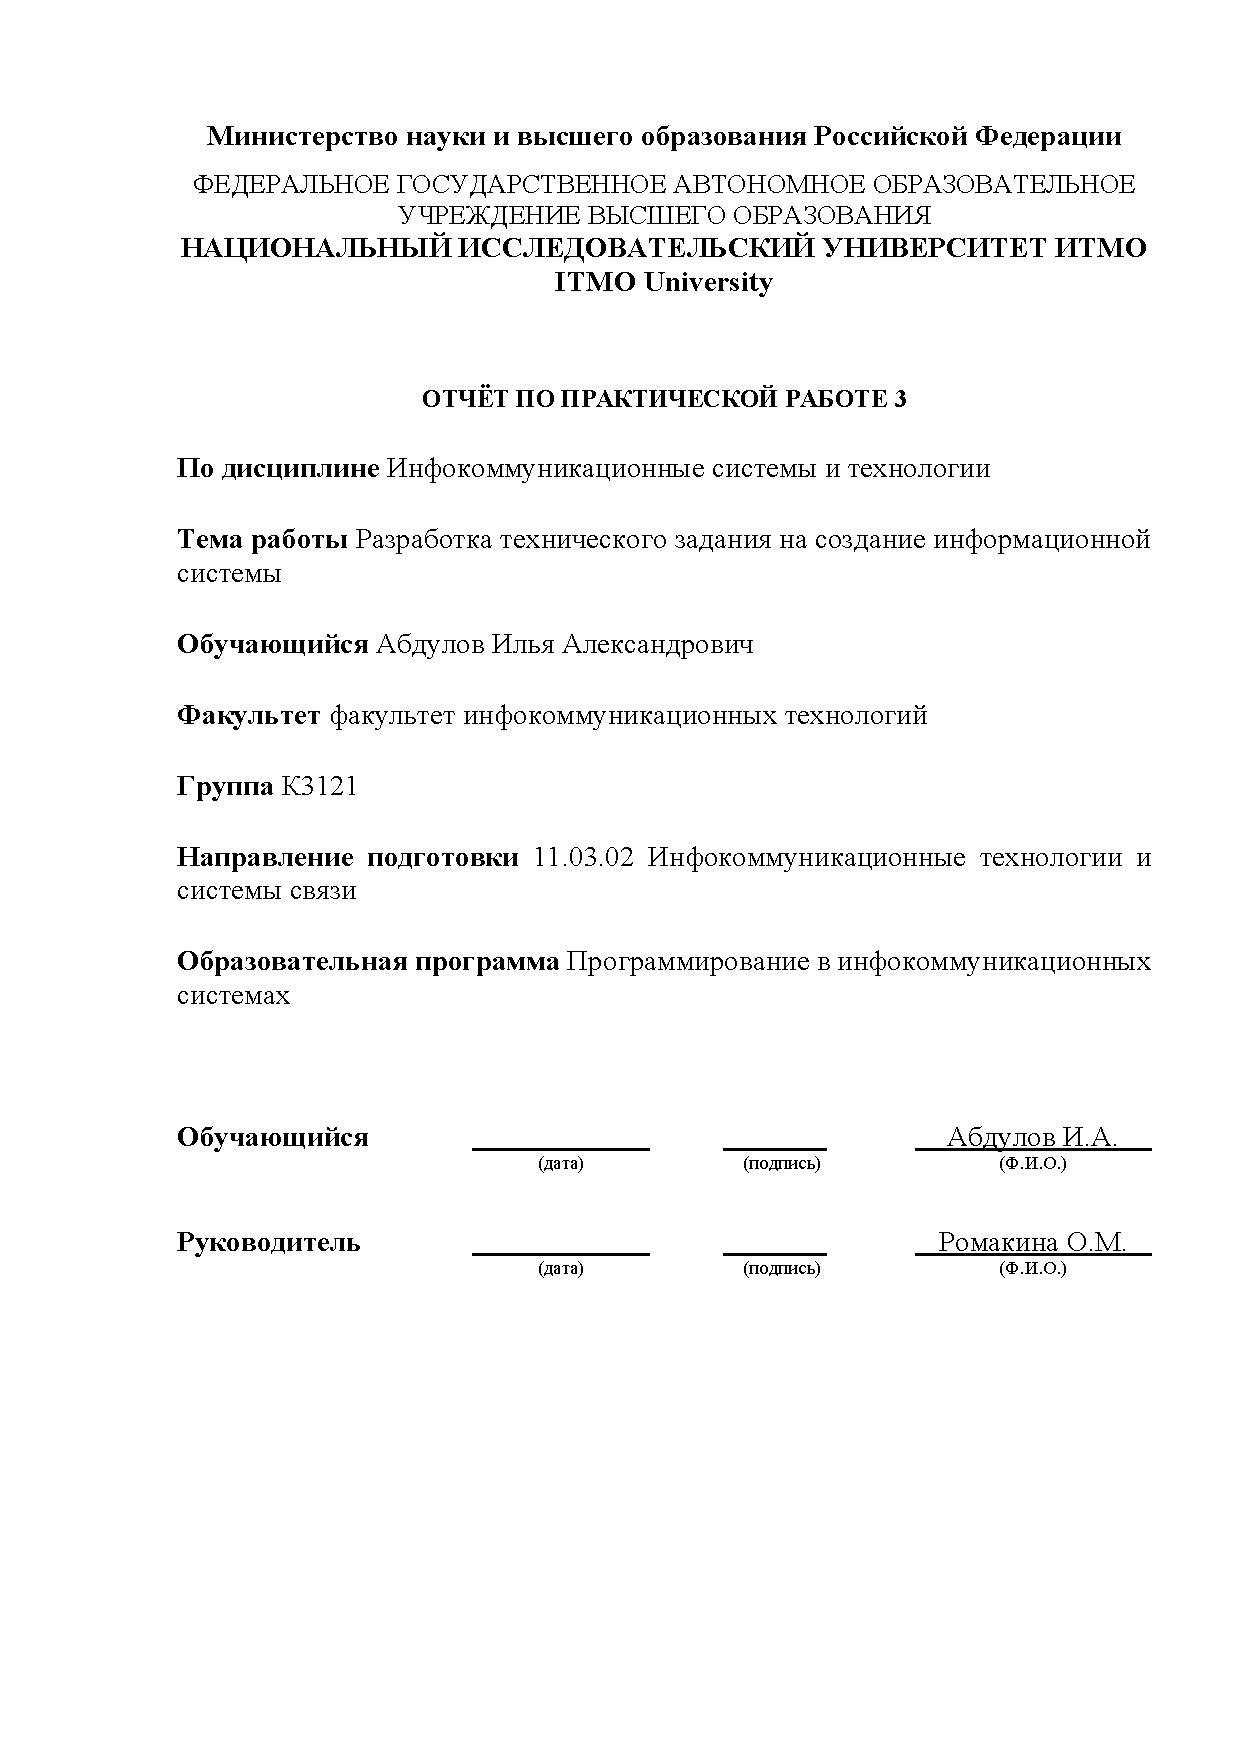
\includepdf{titulCourse.pdf}
\pagestyle{plain}

\tableofcontents

\intro

Практическая работа 5 является актуальной, потому что является описанием основных функциональных элементов будущего мобильного приложения. Приложение Better Row представляет из себя приложение, куда пользователь заносит данные своих тренировок, чтобы приложение показывало и сохраняло текущие показатели и прогресс. Использование приложения придаст тренировкам осознанности, что поможет в достижении лучшего результата.

Целью данной работы является описание предметной области функционирования и основных пользователей будущего мобильного приложения, используя диаграммы UML. В процессе работы будет использован инструмент для создания диаграмм StarUML.

\chapter{Основная часть}

\section{Предметная область функционирования}

Приложение предназначено для развития спортивной деятельности в университете ИТМО, оно предназначено для клуба по академической гребли. Приложение позволяет сохранять данные о тренировке для дальнейшего анализа.

\section{Основные пользователи}

Основными пользователями системы будут являться любители академической гребли и участники студенческой гребной лиги России.

\section{UML диаграммы}

\begin{figure}[H]
\centerline{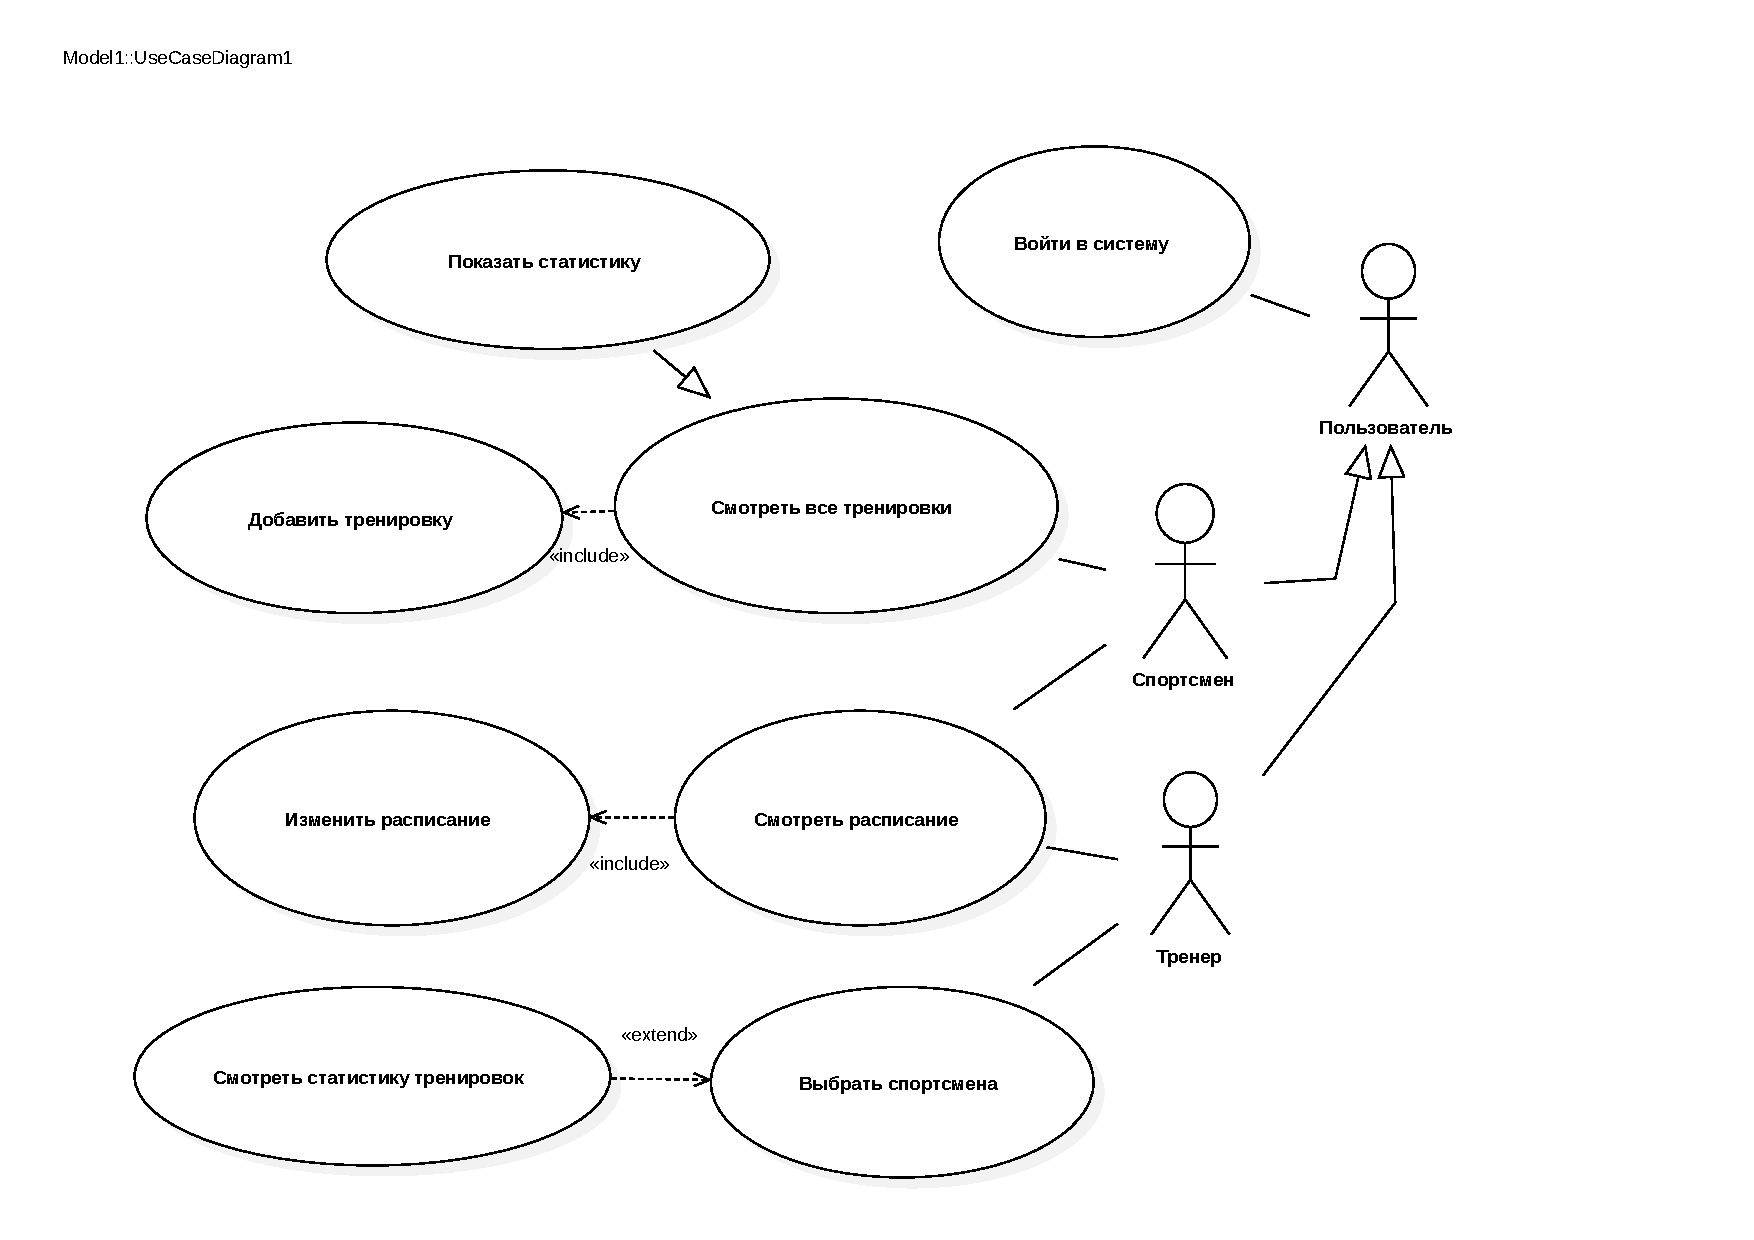
\includegraphics[width=1.2\linewidth]{UseCaseDiagram.pdf}}
\caption{Диаграмма вариантов использования}
\label{fig11}
\end{figure}

\begin{figure}[H]
\centerline{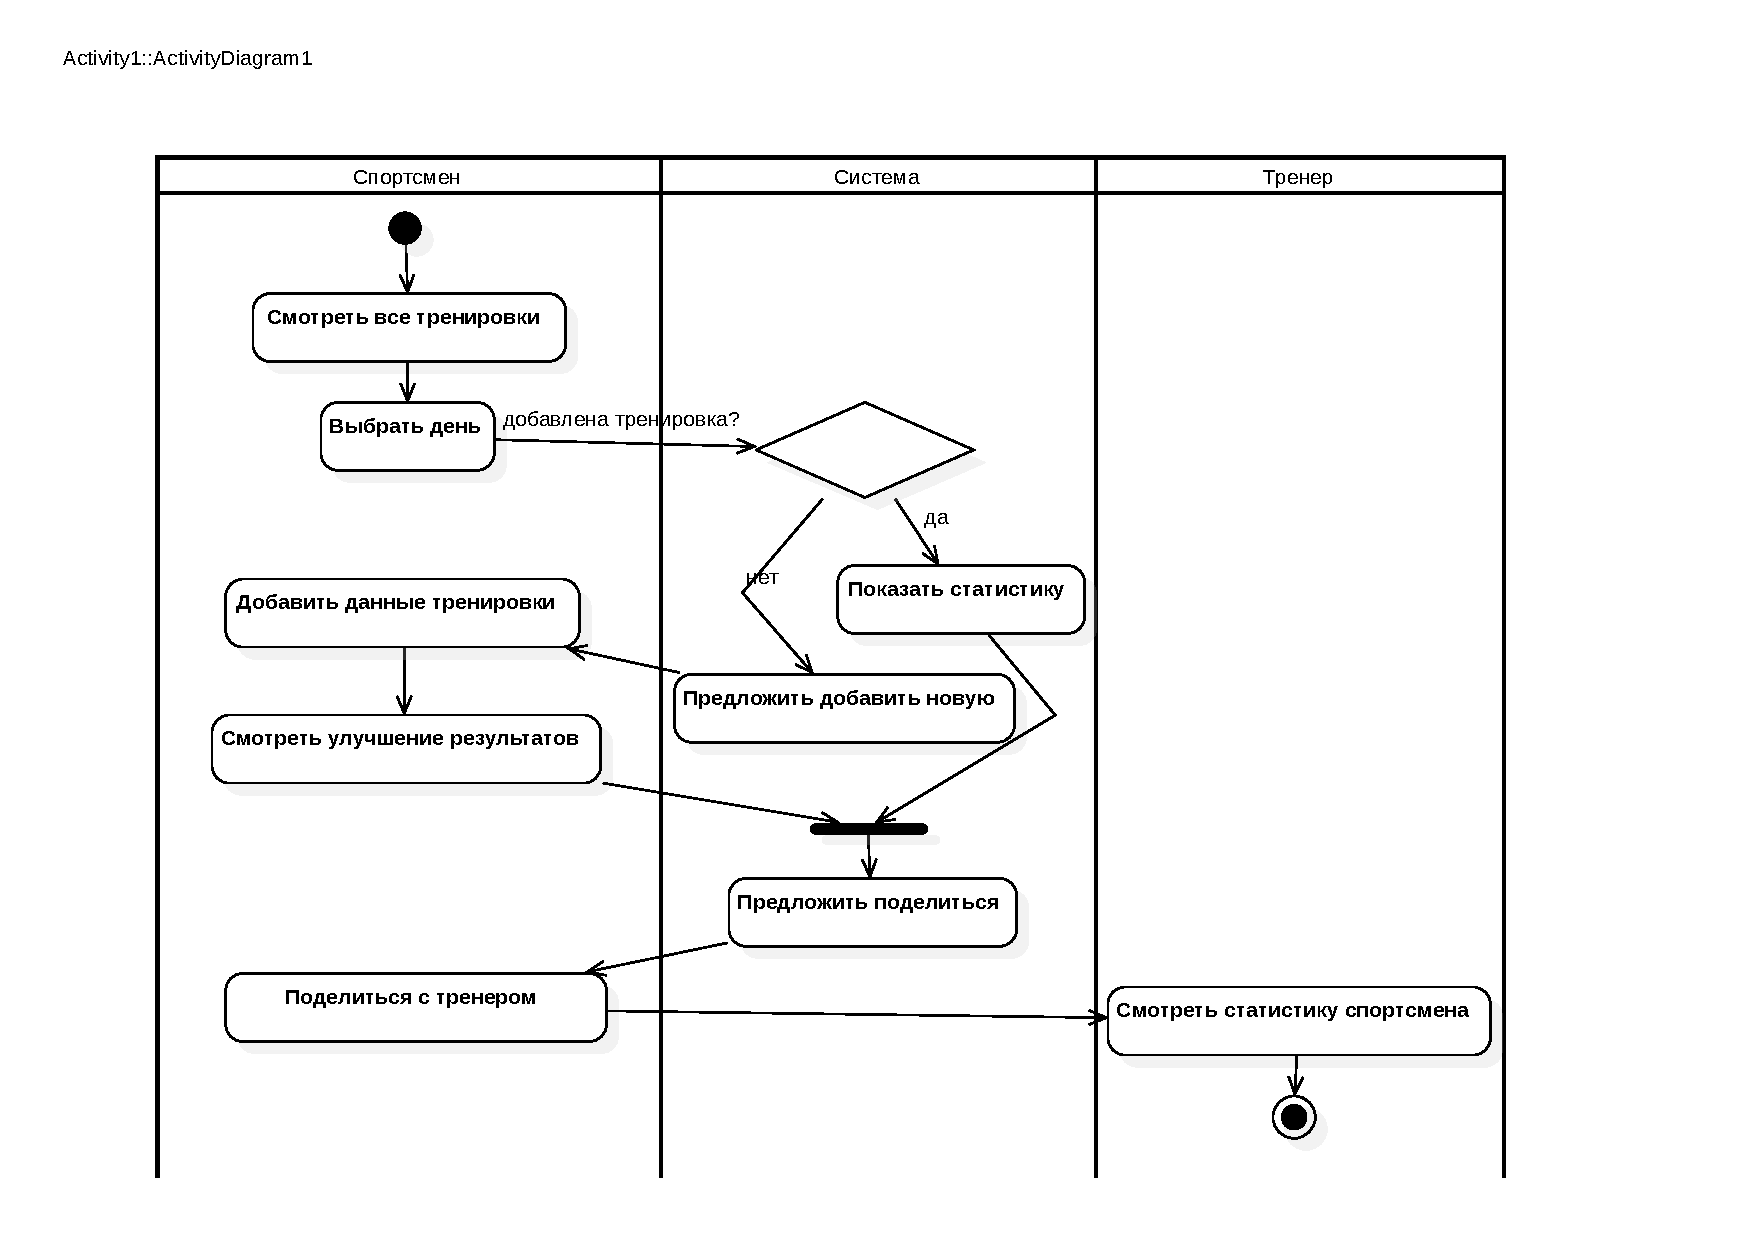
\includegraphics[width=1.2\linewidth]{ActivityDiagram.pdf}}
\caption{Диаграмма активности для ключевого прецедента}
\label{fig12}
\end{figure}

\begin{figure}[H]
\centerline{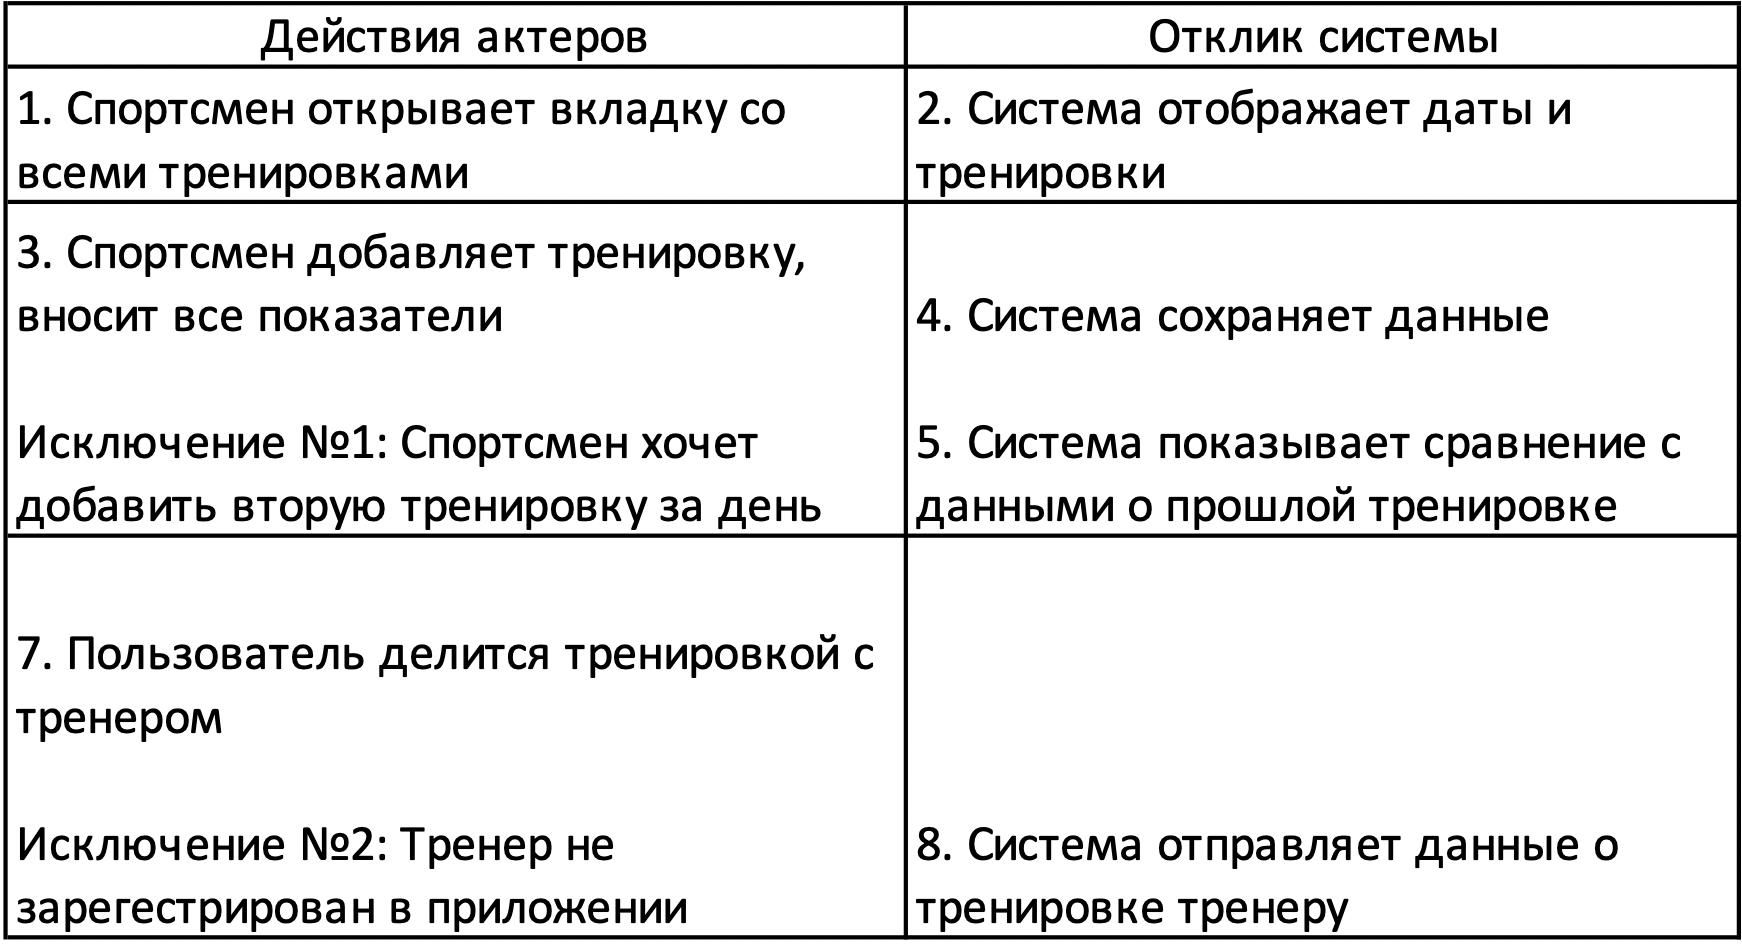
\includegraphics[width=1\linewidth]{Альтернативные потоки.png}}
\caption{Типичный ход события сценария выполнения варианта использования}
\label{fig13}
\end{figure}

\begin{figure}[H]
\centerline{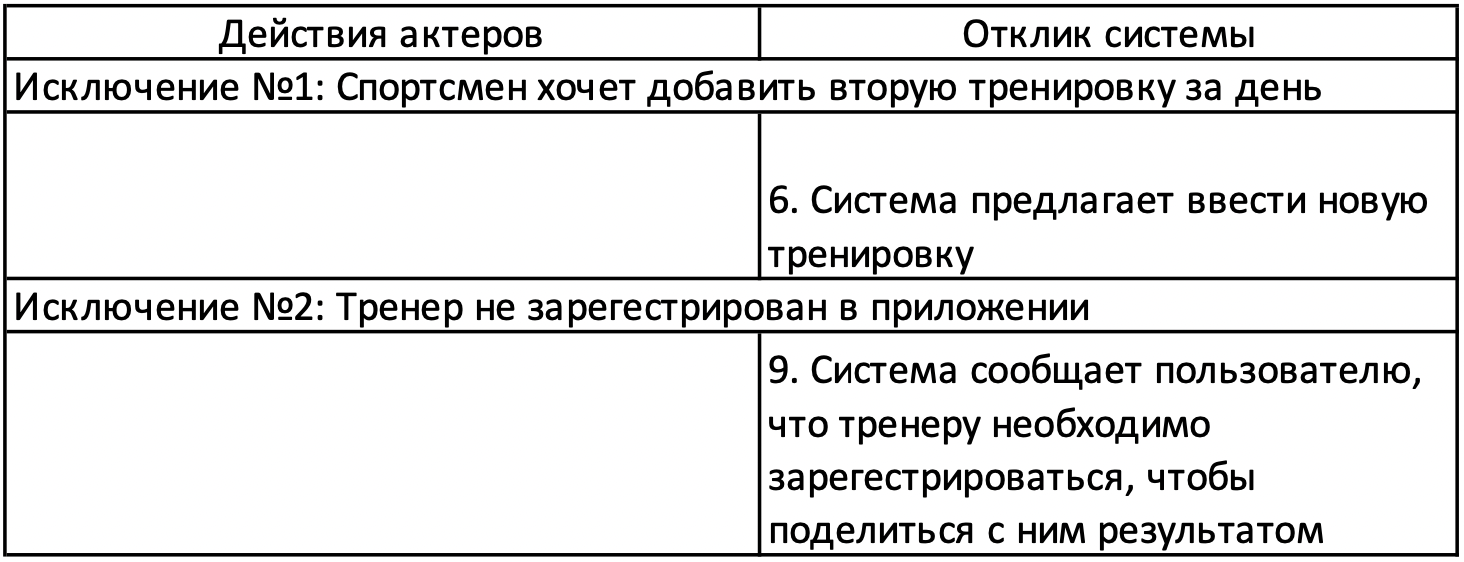
\includegraphics[width=1\linewidth]{Исключения.png}}
\caption{Исключения сценария выполнения варианта использования}
\label{fig14}
\end{figure}

\conclusions

Цель работы была достигнута. Была описана предметная область функционирования, представлены пользователи будущего мобильного приложения. В отчёте были представлены диаграммы вариантов использования, активности для ключевых прецедентов и рассмотрены альтернативные потоки событий.

\newpage
\begin{thebibliography}{99}

\bibitem{bib1}Приложение StarUML для создания UML диаграмм — URL: \url{https://staruml.io/} (дата обращения 03.11.2022).	

\bibitem{bib2}Документация к StarUML — URL: \url{https://docs.staruml.io/} (дата обращения 02.11.2022).	

\bibitem{bib3}Интернет-статья по диаграммам вариантов использования в языке UML — URL: \url{http://sp.cs.msu.ru/ooap/exerb2019.html} (дата обращения 03.11.2022).	
	
\end{thebibliography}

\end{document}
